%%%%%%%%%%%%%%%%%%%%%%%%%%%%%%%%%%%%%%%%%%%%%%%%%%%%%%%%%%%%%%%%%%%%%%%%%%%%%%%%
%2345678901234567890123456789012345678901234567890123456789012345678901234567890
%        1         2         3         4         5         6         7         8

\documentclass[letterpaper, 10 pt, conference]{ieeeconf}  % Comment this line out if you need a4paper

%\documentclass[a4paper, 10pt, conference]{ieeeconf}      % Use this line for a4 paper

%\IEEEoverridecommandlockouts                              % This command is only needed if 
                                                          % you want to use the \thanks command

\overrideIEEEmargins                                      % Needed to meet printer requirements.

% See the \addtolength command later in the file to balance the column lengths
% on the last page of the document

% The following packages can be found on http:\\www.ctan.org
%\usepackage{graphics} % for pdf, bitmapped graphics files
%\usepackage{epsfig} % for postscript graphics files
%\usepackage{mathptmx} % assumes new font selection scheme installed
%\usepackage{times} % assumes new font selection scheme installed
%\usepackage{amsmath} % assumes amsmath package installed
%\usepackage{amssymb}  % assumes amsmath package installed
\usepackage{graphicx} % for pdf, bitmapped graphics files
\usepackage{float}
\usepackage{caption}
\usepackage{subcaption}
%\usepackage{algorithm,algpseudocode}

%\usepackage{epsfig} % for postscript graphics files
%\usepackage{mathptmx} % assumes new font selection scheme installed
%\usepackage{times} % assumes new font selection scheme installed
\usepackage{amsmath} % assumes amsmath package installed
%\usepackage{amssymb}  % assumes amsmath package installed
\usepackage{enumerate}

\title{Project Report:\\\LARGE \bf
Stereo Matching using Graphcut-based Optimization}

\author{Seyed Abbas Sadat\\
Simon Fraser University\\
sas21@sfu.ca% <-this % stops a space
}


\begin{document}



\maketitle
\thispagestyle{empty}
\pagestyle{empty}

%%%%%%%%%%%%%%%%%%%%%%%%%%%%%%%%%%%%%%%%%%%%%%%%%%%%%%%%%%%%%%%%%%%%%%%%%%%%%%%%

\section{INTRODUCTION}

\begin{figure*}[t]
        \centering
        \begin{subfigure}[b]{0.3\textwidth}
                \centering
                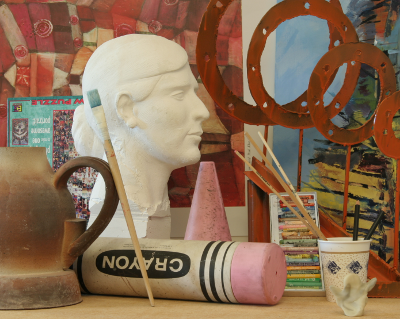
\includegraphics[width=\textwidth]{imgs/l4.png}
                \caption{"Art" Color image}
                \label{fig:trees}
        \end{subfigure}%
                ~ %add desired spacing between images, e. g. ~, \quad, \qquad etc.
          %(or a blank line to force the subfigure onto a new line)
        \begin{subfigure}[b]{0.3\textwidth}
                \centering
                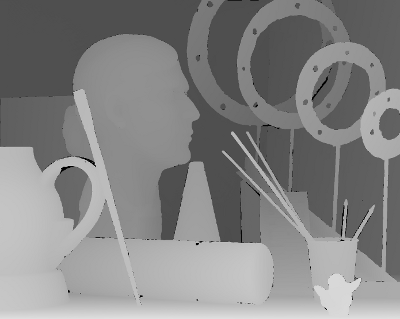
\includegraphics[width=\textwidth]{imgs/disp4.png}
                \caption{Ground Truth}
                \label{fig:farm}
        \end{subfigure}
                ~ %add desired spacing between images, e. g. ~, \quad, \qquad etc.
          %(or a blank line to force the subfigure onto a new line)
        \begin{subfigure}[b]{0.3\textwidth}
                \centering
                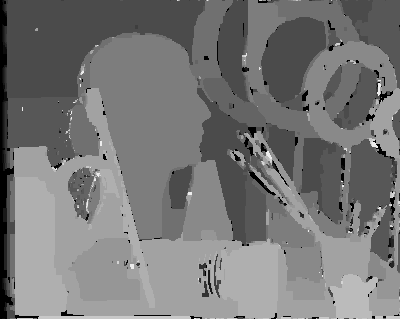
\includegraphics[width=\textwidth]{imgs/l4disparity-expansion.png}
                \caption{$\alpha$-expansion}
                \label{fig:farm}
        \end{subfigure}
                ~ %add desired spacing between images, e. g. ~, \quad, \qquad etc.
          %(or a blank line to force the subfigure onto a new line)
        \begin{subfigure}[b]{0.3\textwidth}
                \centering
                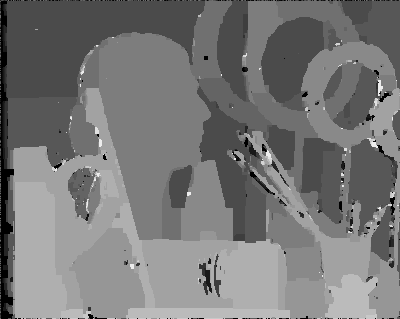
\includegraphics[width=\textwidth]{imgs/l4disparity-swap.png}
                \caption{$\alpha\beta$-swap}
                \label{fig:farm}
        \end{subfigure}
                        ~ %add desired spacing between images, e. g. ~, \quad, \qquad etc.
          %(or a blank line to force the subfigure onto a new line)
        \begin{subfigure}[b]{0.3\textwidth}
                \centering
                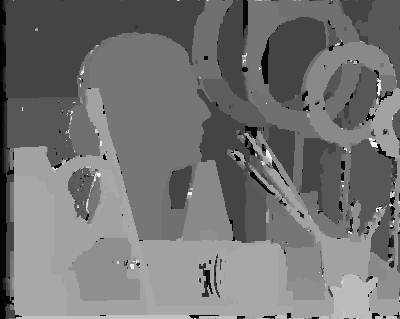
\includegraphics[width=\textwidth]{imgs/l4disparity-expansion-sub.png}
                \caption{$\alpha$-expansion - subpixel accuracy}
                \label{fig:farm}
        \end{subfigure}
                ~ %add desired spacing between images, e. g. ~, \quad, \qquad etc.
          %(or a blank line to force the subfigure onto a new line)
        \begin{subfigure}[b]{0.3\textwidth}
                \centering
                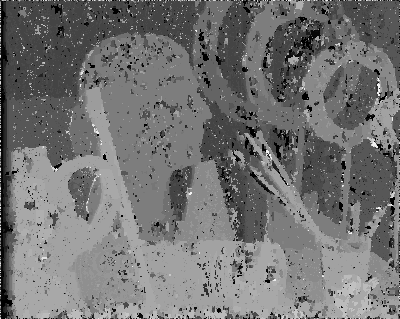
\includegraphics[width=\textwidth]{imgs/l4disparity-swap-sub.png}
                \caption{$\alpha\beta$-swap - subpixel accuracy}
                \label{fig:farm}
        \end{subfigure}
        \caption{Disparity image for the "Art" dataset using the both $\alpha\beta$-swap and $\alpha$-expansion with pixel and subpixel accuracies.}
        \label{fig:realmaps}
\end{figure*}

\begin{figure*}[t]
        \centering
        \begin{subfigure}[b]{0.3\textwidth}
                \centering
                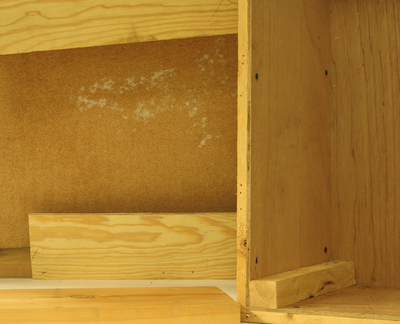
\includegraphics[width=\textwidth]{imgs/l2.png}
                \caption{"Wood1" Color image}
                \label{fig:trees}
        \end{subfigure}%
                ~ %add desired spacing between images, e. g. ~, \quad, \qquad etc.
          %(or a blank line to force the subfigure onto a new line)
        \begin{subfigure}[b]{0.3\textwidth}
                \centering
                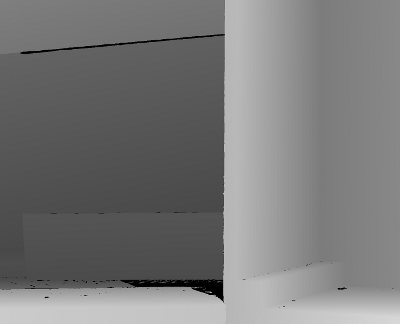
\includegraphics[width=\textwidth]{imgs/disp2.png}
                \caption{Ground Truth}
                \label{fig:farm}
        \end{subfigure}
                ~ %add desired spacing between images, e. g. ~, \quad, \qquad etc.
          %(or a blank line to force the subfigure onto a new line)
        \begin{subfigure}[b]{0.3\textwidth}
                \centering
                
\includegraphics[width=\textwidth]{imgs/l2disparity-expansion.png}
                \caption{$\alpha$-expansion}
                \label{fig:farm}
        \end{subfigure}
                ~ %add desired spacing between images, e. g. ~, \quad, \qquad etc.
          %(or a blank line to force the subfigure onto a new line)
        \begin{subfigure}[b]{0.3\textwidth}
                \centering
                
\includegraphics[width=\textwidth]{imgs/l2disparity-swap.png}
                \caption{$\alpha\beta$-swap}
                \label{fig:farm}
        \end{subfigure}
                        ~ %add desired spacing between images, e. g. ~, \quad, \qquad etc.
          %(or a blank line to force the subfigure onto a new line)
        \begin{subfigure}[b]{0.3\textwidth}
                \centering
                
\includegraphics[width=\textwidth]{imgs/l2disparity-expansion-sub.png}
                \caption{$\alpha$-expansion - subpixel accuracy}
                \label{fig:farm}
        \end{subfigure}
                ~ %add desired spacing between images, e. g. ~, \quad, \qquad etc.
          %(or a blank line to force the subfigure onto a new line)
        \begin{subfigure}[b]{0.3\textwidth}
                \centering
                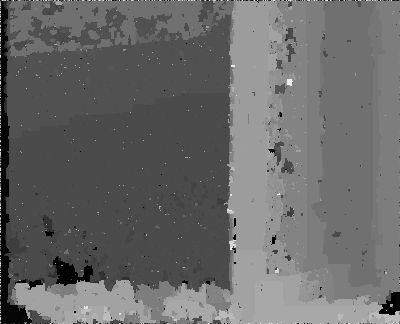
\includegraphics[width=\textwidth]{imgs/l2disparity-swap-sub.png}
                \caption{$\alpha\beta$-swap - subpixel accuracy}
                \label{fig:farm}
        \end{subfigure}
        \caption{Disparity image for the "Wood1" dataset using the both $\alpha\beta$-swap and $\alpha$-expansion with pixel and subpixel accuracies.}
        \label{fig:realmaps}
\end{figure*}

In this project we developed a stereo matching system based on graph-cut optimization framework \cite{boykov2001fast}. In stereo matching problem, 2 images taken from 2 cameras that are in the same hozirontal like The input to the system is a pare of images 

\section{Graphcut-based Optimization}
\section{Stereo Matching}
\section{Experiments and Results}
\bibliographystyle{ieeetr} 
\bibliography{refs}


\end{document}
